%Chapter 7 - What is required to bring the MEGA65 to a MVP and market?
%What is required to bring the MEGA65 to a MVP and market?

\chapter{What is required to bring the MEGA65 to a MVP and market?}
\label{Chapter7}
This chapter discusses the possible features the MEGA65 should included to meet the expectations and needs of users. It looks at both form-factors of the MEGA65, the hand-held console and well as the desktop computer form-factor. After listing the features likely to be wanted by users and determining a MVP (Minimum Viable Product), this chapter discusses the work needed to be done to bring the MEGA65 to the stage of a MVP.

%----------------------------------------------------------------------------------------
%----------------------------------------------------------------------------------------

\section{Use cases}
This sections lists and discusses use cases for the MEGA65 in both its form-factors, the desktop computer and the hand-held console. By studying the way the MEGA65 might possibly be used and extracting the features required to fur fill each use case and then ranking them in order of importance, it is possible to create a list of features will be of high value to users of the MEGA65. This list can then help with decision making regarding the MVP of the MEGA65. The use cases where first decided upon by determining some roles or actors from the MEGA65's target market. These actors are described below, as well as a brief look at there likely use cases as seen in figure \ref{MEGA65_use_cases}. It can be concluded from this that as a large portion of the target market would appreciate the features which support the playing of retro games and applications, then a focus on those features would be recommended for the MVP.

\textbf{Gamer}
The Gamers goal is to be able to play retro games. The amount of games and the ability to add more games as well as controller options such as an external joystick are all important to this actor.

\textbf{8-bit Programmer}
The 8-bit Programmer referred to as just Programmer from here on, has a goal of being able to run 8-bit programs in a C64 or C65 environment. They are interested in any features which will add compatibility such as support for different opcodes or new video modes. 

\textbf{Tech Enthusiast}
The Tech Enthusiast's goal is to try new technology and experience rare or peculiar technological devices, this group also contains 'modders' or 'hackers', people that like to change products they have been purchased. They are interested in any of the features but especially in the features that will add something unique or the ability to modify the product easily.

\textbf{Privacy Motivated}
The Privacy Motivated actor's goals is to be able to securely communicated and carry out a variety of tasks. They are interested in features that will let them thwart any malicious attempts to obtain data. Features that will allow the actor to perform check as increase trust of the security of the device will also be highly valued. 

\begin{figure} \begin{center}
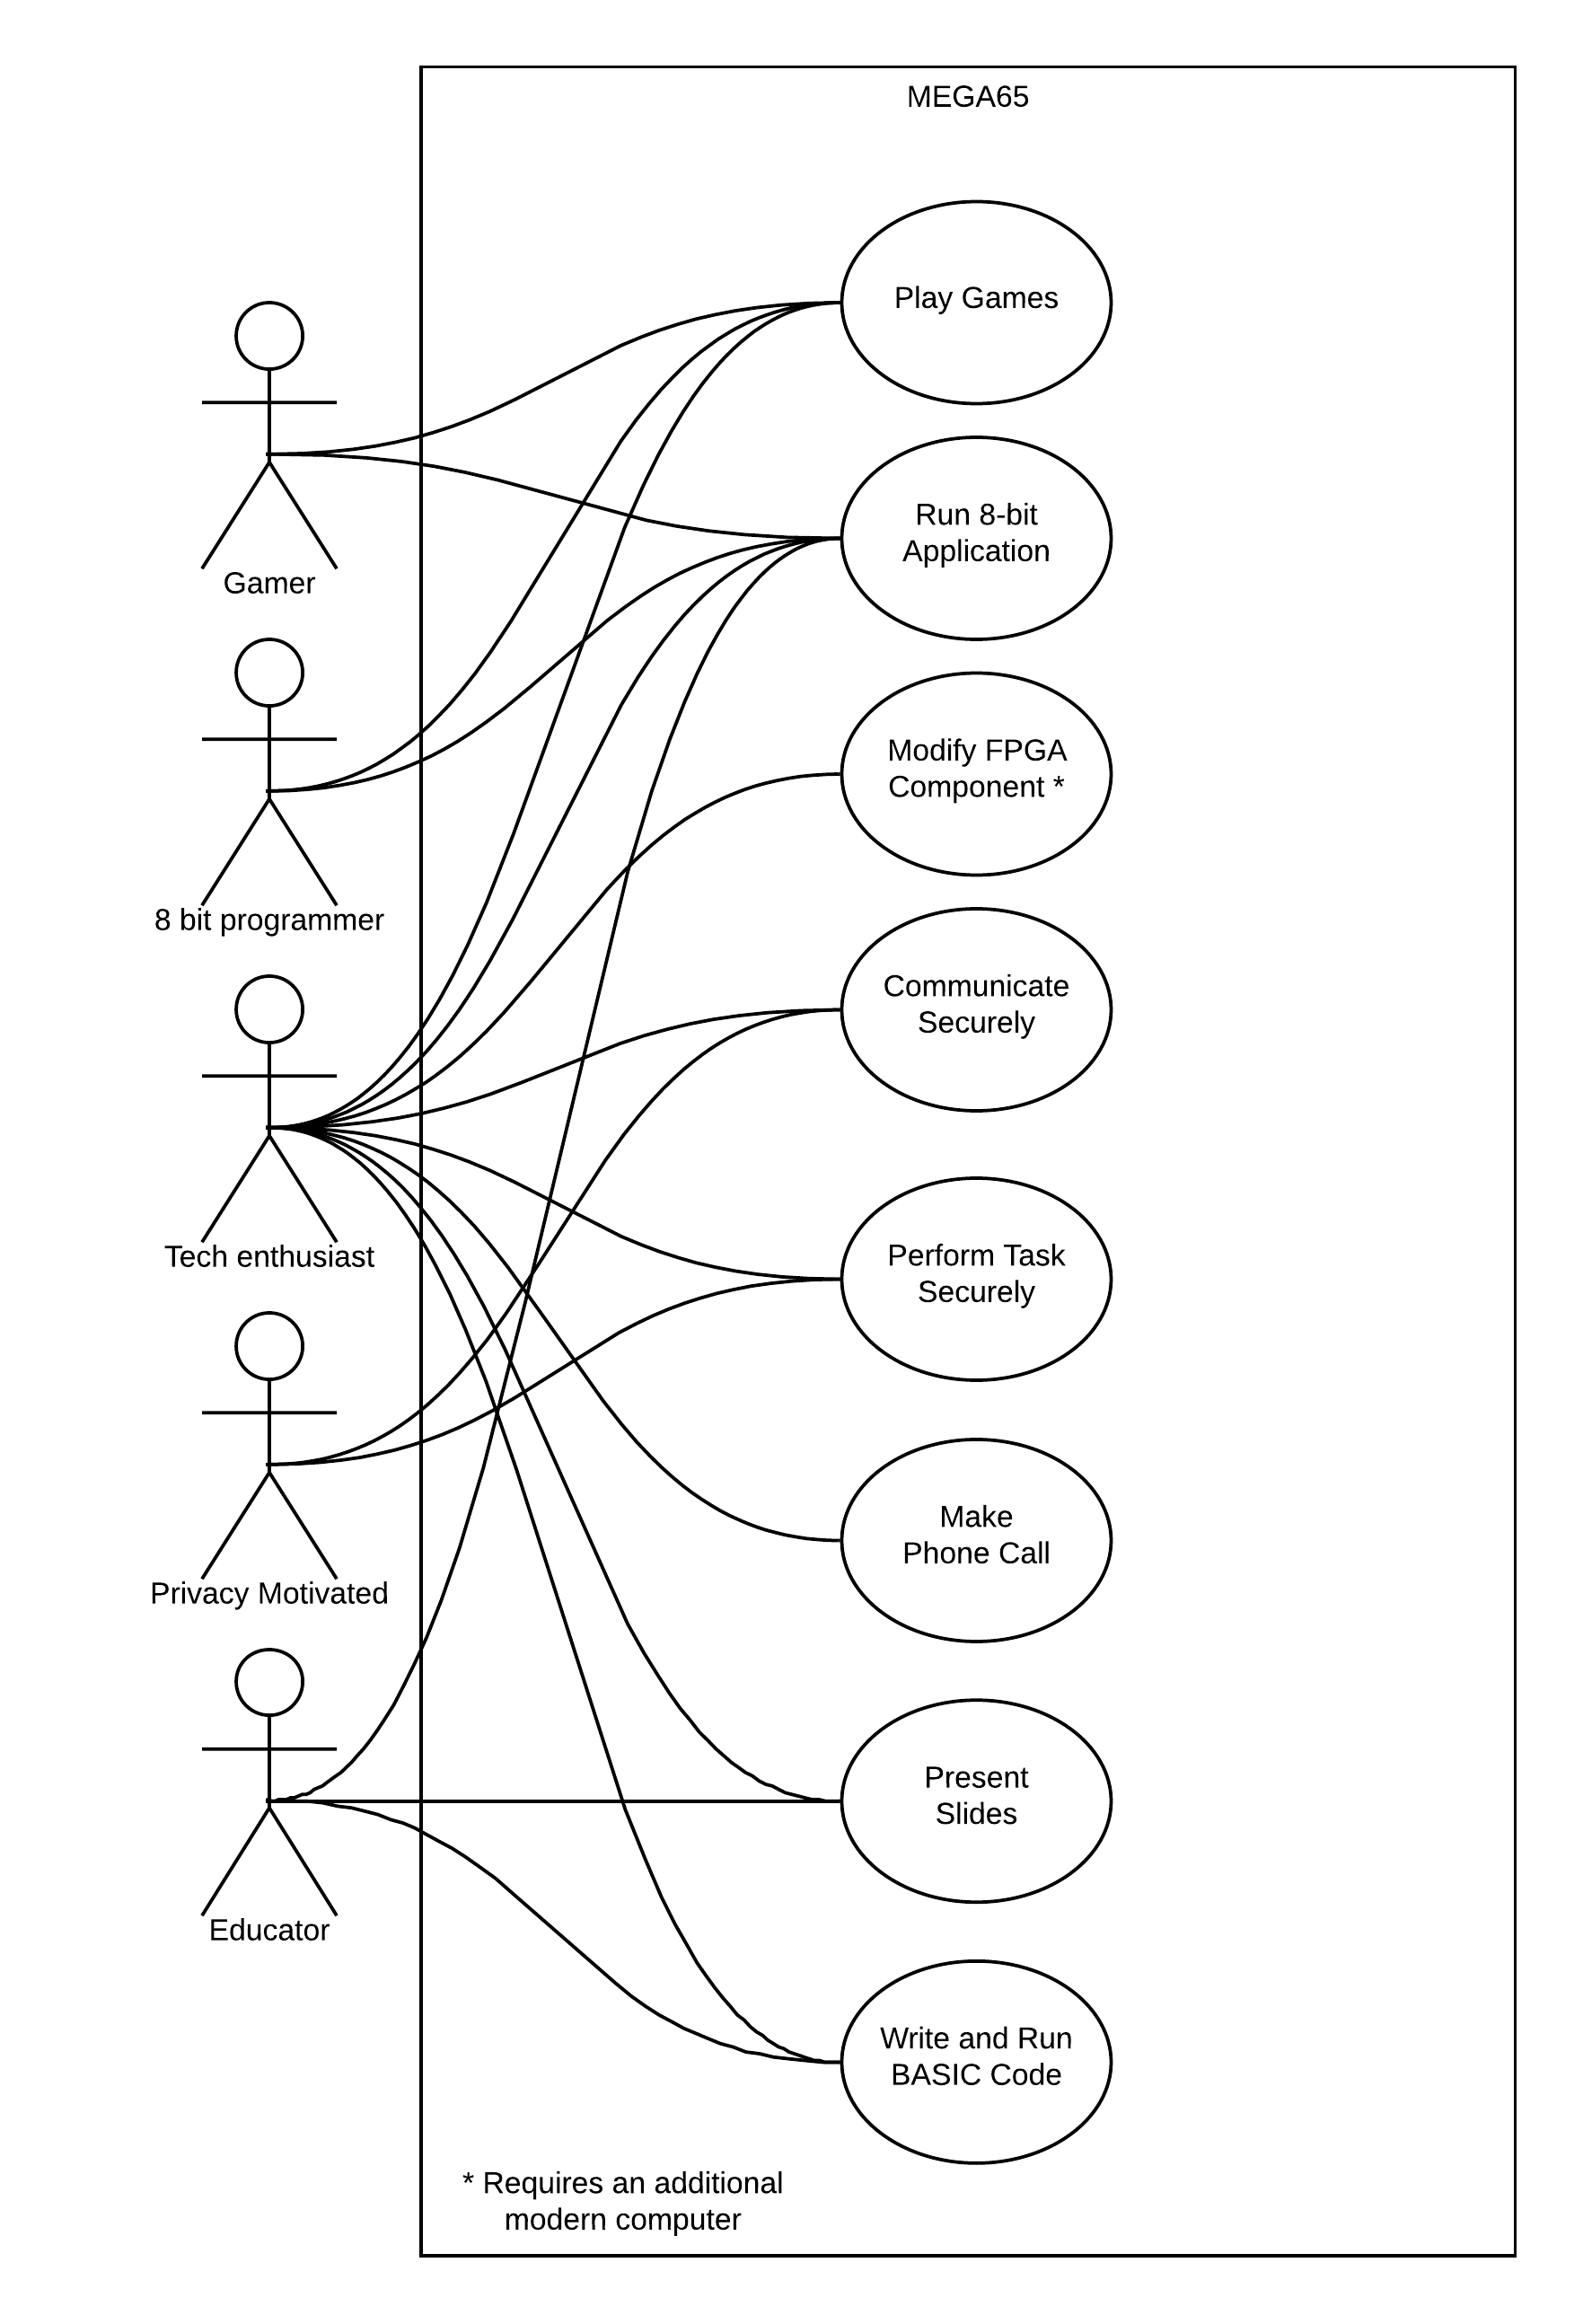
\includegraphics[width=.6\linewidth]{pics/MEGA65_use_case} 
\end{center} 
\caption{MEGA65 Use Cases for the target market\\}
\label{MEGA65_use_cases}
\end{figure}

\section{PCB}
The PCB or motherboard will house the FPGA as well as the other electrical components including the ports. This is an essential component. The exact design  will differ between the two form factors due to several constraints and influences, not least of which the fact that they are being developed by two different teams with vastly different levels of experience. The PCB is closely bound to a large range of features as it is necessary to change the PCB design to account for many of them.

\section{Case}
The case will be necessary for ascetic reasons as well as quality and performance issues relating to ingress dust etc. There may also be some regulatory issues around not having a case but the market reasons are sufficient alone to warrant one. The case will be different for each form-factor of the MEGA65, as they are to be different sizes. The case will likely have to be changed for any new control or ports but besides that most features will not effect the case. This doesn't include case-related features of course, such as ergonomic hand holds.


\section{Keyboard/Buttons}
The keyboard and buttons are quite essential to the MVP for obvious reasons. The MEGAphone form factor will not feature a keyboard as it is a held held device, a keyboard would require to much space as well as not being essential to using the MEGAphone for most of its intended uses, such as playing games. The desktop form factor should have a full-sized keyboard as a desktop form-factor has the luxury of being able to be larger, the original Commodore computers featured a keyboard and as this is based off them cstomers will expect a keybaord. A keyboard all adds convieanace when trying to perform complex tasks on the MEGA65, such as coding.


\section{Regulatory Approvals}

\section{Packaging}

\section{Documentation}

\section{Firmware}

\section{Bundled Software}

\section{Commodore 65 ROM Licenses}


From Paul - 
Some things potentially needed for an MVP: Case, keyboard, motherboard, regulatory approvals, packaging, user/setup guide, firmware, bundled software, C65 ROM license.

